%!TEX root = thesis.tex
Our second prototype will move away from the world of jammable shape changing interfaces and into the surfaces of our environment.
Since the vision of ubiquitous computing was presented researchers have sought to integrate interactive technology into our everyday environment in variety of ways, which can be seen from the diverse selection of research fields that has stemmed from ubiquitous computing such as context awareness, tangible computing and shape changing interfaces.
In this prototype we have taken Weiser's vision very literally - how do you integrate interaction into the fabric of our everyday environment, i.e. the surfaces that surrounds us?

In the following sections we explore the possibilities of creating textile touch surfaces with advanced interaction capabilities as an exemplification of how surfaces can be used to interact in the home.
We have chosen to work with textiles as an interactive platform as we see unused potential in this area, both for its tangible and aesthetic textural qualities compared to e.g. polymer solutions \cite{rosenberg2009unmousepad}, as well as for the interesting possibilities to allow for DIY solutions to creating interactive stuff in the home.

\section{Related work and approaches}
Before getting into detail with our implementation we will first give an overview of work and approaches that relates to our prototype and have inspired our solution.
We are, of course, not the first ones to consider the surfaces that surrounds us as interactive potential.
For example interactive floors such as iFloor \citep{petersen2005floor} and  iGameFloor \citep{gronbaek2007igamefloor}, augmented surface displays in fridges, walls and bowls \citep{taylor2007homes}, interactive tables such as reacTable \citep{jorda2007reactable} or, quite different from the other examples, REVEL that via a digital overlay changes the tactile perception of a physical surfaces \citep{bau2013revel}.

We have separated this section into three different fields that all have influenced the construction and implementation of our prototype work: electronic textiles, touch sensing and gesture recognition.
 
\subsection{Electronic Textiles}
\begin{quotation}
\emph{The most profound technologies are those that disappear. They weave themselves into the fabric of everyday life until they are indistinguishable from it. \citep{weiser1991computer}}
\end{quotation}
One of the research areas that have stemmed from ubiquitous computing is electronic textiles or `e-textiles', which seeks to integrate electronic and computation into fabric.
\citet{park2002wearable} presents the E-Textile vision as the paradigm the ``fabric is the computer'', taking Weiser's much quoted description of ubiquitous computing very literal.
One of the main obstacles for attaining this vision of the \emph{fabric as the computer} is how to incorporate the underlying computation into the fabric.
There are generally seen three ways to do it, either by computing \emph{offline}, on a separate system connected to the fabric, \emph{onto}, on components attached to the fabric or \emph{into} the fabric, embedded seamlessly into it \citep{marculescu2003}.
Today computation is commonly done either offline or onto the fabric, or a combination of the two, but advances in organic electronics and nano technology, for example with organic transistors weaved into fabric \citep{lee2005weave}, suggests that computation embedded into the fabric is not far off.
\begin{figure}
\centering
\begin{minipage}[t]{.3\textwidth}
  \centering
  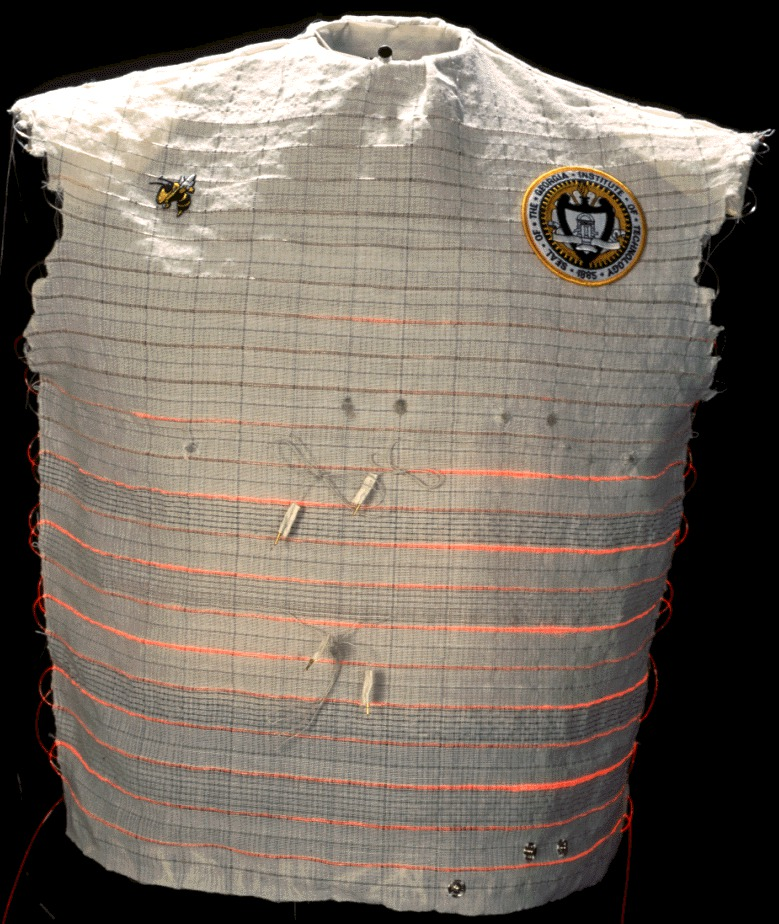
\includegraphics[width=0.8\linewidth]{figures/wearable_motherboard}
  \captionof{figure}{The Wearable Motherboard, taken from \citep{gopalsamy1999wearable}}
  \label{sofa_interaction:wearable_motherboard}
\end{minipage}%
\hspace{0.2cm}
\begin{minipage}[t]{.3\textwidth}
  \centering
  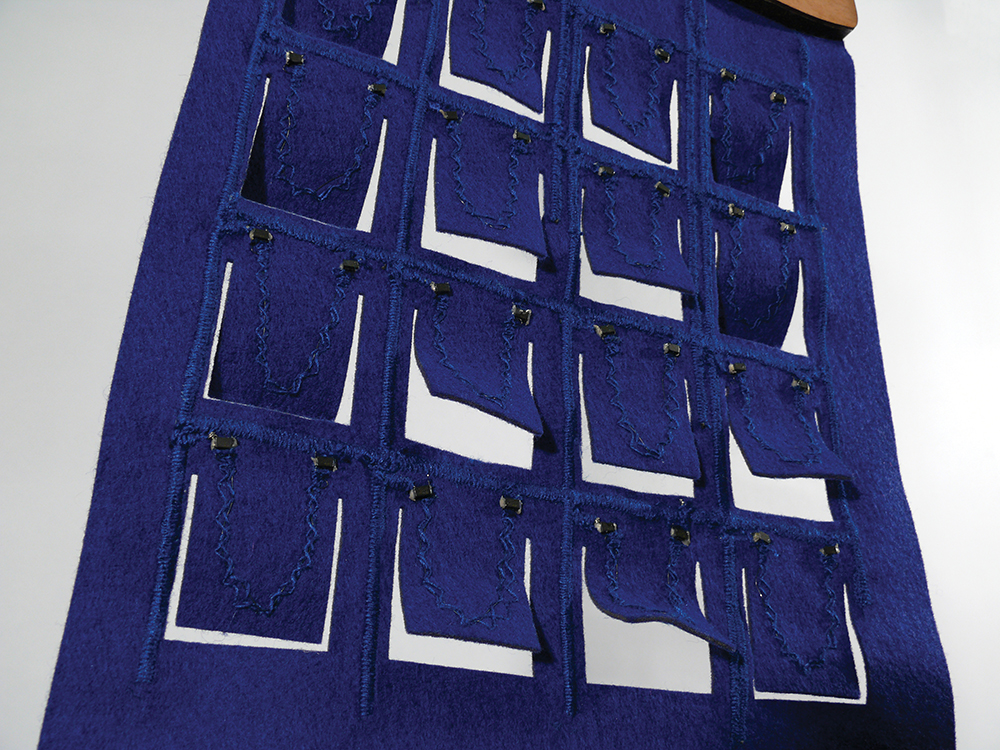
\includegraphics[width=0.8\linewidth]{figures/shutters}
  \captionof{figure}{Shutters, taken from \citep{coelho2009shutters}}
  \label{sofa_interaction:shutters}
\end{minipage}
\hspace{0.2cm}
\begin{minipage}[t]{.3\textwidth}
  \centering
  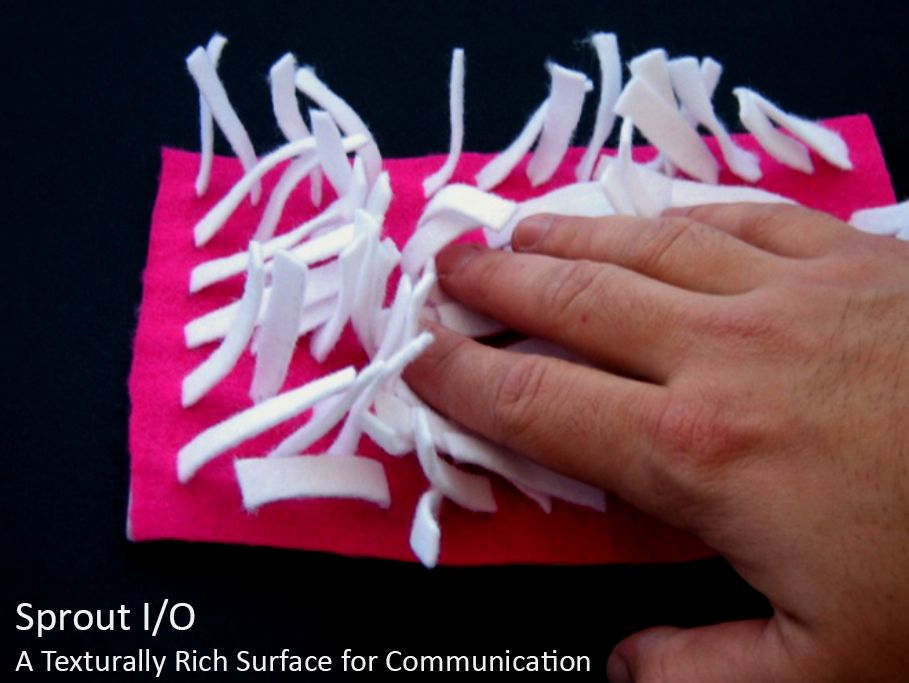
\includegraphics[width=0.8\linewidth]{figures/sprout}
  \captionof{figure}{Sprout I/O, taken from \citep{coelho2009shutters}}
  \label{sofa_interaction:sprout}
\end{minipage}
\end{figure}
E-textile is often seen used as part of wearable computing systems, logically, since clothing as a medium is ever present when people are involved.
An example of this is the Wearable Motherboard \citep{gopalsamy1999wearable} seen in figure~\ref{sofa_interaction:wearable_motherboard}, also called the ``Smart Shirt'', which is a lightweight monitoring `shirt' that can provide sensory data for use in medical and military contexts.
The fabric here is used as data paths that facilitates routing of information from any point to any other point on the shirt through conductive fibers embedded in the fabric.

E-textiles are not limited to wearable computing and clothing, and can just as well be part of interior design such as curtains, pillows, carpets, upholstery ect.
Shutters by \citet{coelho2009shutters}, seen in figure~\ref{sofa_interaction:shutters}, is an example of this where shape-memory alloy (SMA) threads are woven into a felt surface creating a curtain-like structure capable change of shape in permeability, used for indoor ventilation control among other things.
Here the SMA allows for actuation in the shutters while retaining the look, feel and softness of textile without any hard mechanic actuators.  
Another example from \citet{coelho2008sprout} is Sprout I/O, see figure~\ref{sofa_interaction:sprout}, where a membrane filled with strands of SMA and felt provides textually rich input and actuated output capabilities.
By measuring the capacitance between the users hand and the SMA threads touches can be registered, enabling stroke-like interaction, by creating an input matrix that register changes in each of the the individual SMA threads.

We have gotten a lot of inspiration from the various ``Do It Yourself'' (DIY) on-line communities related to e-textile craft and crafts in general, notably KOBAKANT DIY \citep{kobakantWEB} and Instructable \citep{instrucableWEB}.
Both sites provides guides, tips, and tricks for materials, construction and techniques and have for us been a good starting point for doing an e-textile project.
One of our inspirations has been rSkin \citep{rskinplusea,rSsininstructables}, a project by Hannah Perner-Wilson, which attempts to create a `skin' for a robot arm, made out of textiles, that enables the arm to register intensity and location of touches on the whole arm, seen in figure~\ref{rskin}.

\begin{figure}[hb]
	\centering
  		\includegraphics[width=3in]{figures/rskin}
	\caption[rSkin, Open Source Robot Skin]
   {rSkin, Open Source Robot Skin}
   \label{rskin}
\end{figure}
The `skin' is made of stretchy fabric and a 28 rows x 28 columns large pressure sensitive grid is embedded into the fabric using conductive thread.
The skin is made out of three layers: first a non-conductive layer with 28 rows of conductive thread, then a layer piezoresistive fabric and lastly a non-conductive layer with 28 columns of conductive thread.
The piezoresistive fabric acts as a pressure sensitive layer as piezoresistive materials decrease their electrical resistivity under mechanical stress \citep{piezoresistiveWIKIPEDIA}.
This approach to making pressure sensitive grids will be described in further detail in the implementation section as we use it as a starting point for our second prototype iteration.

\subsection{Touch Sensing}
\todo{bedre indledning}

Generally seen there are three broad categories for doing multi-touch input sensing: optical, capacitive and resistive \citep{rosenberg2009unmousepad}.

Optical sensing usually involve one or more digital cameras placed behind the touch surface to generate an image of the user's finger to track the interaction.
As this approach relies on cameras it is typically used for larger applications such as tabletops, since the cameras has to be far enough away to capture entire interactive surface, e.g. reacTable \citep{jorda2007reactable} and the tabletop version of Microsoft Surface.

Capacitive sensing systems for touch based interaction rely on the human body's capacitive abilities to acquire the position of the touch on a surface. 
As a finger touches the surface, the surface's electrostatic field distorts and this change is then measurable as a change in capacitance at some position in a 2D grid.
The most common example of this approach is the touch surface of modern smart phones and tablets where touch has become the preferred form of interaction.
Another example is Touch\'e \citep{sato2012touche} that allow objects and environments to become touch sensitive, allowing everyday objects to become touch interfaces, such as doorhandles, cups, water bottles ect.
This is done by sending a signal through the object and doing electromagnetic frequency sweeps. 
These frequencies will change when a touch occur and will change based on the size of the touched on the surface allowing for simple gesture recognition.
Two limitations of this technology is that pressure can not reliably be measured and that most systems based this technology only works with bare skin touching it.    

Resistive sensing is based on the principle of Force Sensitive Resistance (FSR). 
\citet{rosenberg2009unmousepad} describes FSR devices as 
\begin{quotation}
\emph{a continuous electrical switch through which electric conductance increases gradually as external force is applied}
\end{quotation}
The simple approach is to create a discrete array of FSR sensors in which each sensor has its own input and output channel.
This has some obvious limitations that will be discussed in iteration 1 in the next section.
Another approach is to create a row/column grid as seen in previously mentioned rSkin, this approach will be explored in iteration 2.
Lastly in iteration 3 we will explore the approach suggested by \citet{rosenberg2009unmousepad} to create a device based on IFSR, which is interpolating FSR, to increase the resolution of our prototype.
Generally seen resistive sensing is a low-cost and easy to implement solution to doing multi-touch interfaces and has the added benefit of being able to measure pressure.
Though to attain resolutions higher than the size of the underlying grid, a lot of data processing has to be done as seen in \citep{rosenberg2009unmousepad}.
Also from our own experience with the technology we have seen a lot of input signal noise from the sensor which makes it harder to get accurate position tracking.   

\subsection{Gesture recognition}
Being able to sense a x-y position or a pressure map on an interactive surface is usually not enough for an application to provide interesting interaction possibilities.
Adding gestures can be one way to approach the interaction in a more involving, natural and expressive way.
\citet{baudel1993charade} points out three possible advantages in using gesture based systems:
\begin{itemize}
  \item \emph{Natural interaction:} Gestures are a natural and intuitive way to interact that is easy to learn.
  \item \emph{Terse and powerful interaction:} The expressive nature of a gesture can provide the ability for a single gesture to specify both a command and its parameters.
  \item \emph{Direct interaction:} As the hand is used for input no intermediate transducer is needed
\end{itemize}
Gestures inherent expressive character does pose a challenge though as the computer system has to interpret the gesture in some way to give it meaning.
Reversely the user needs to know, or at least have hints at, which gestures that the system understands in order to interact with it.
Some types of gestures and their interaction meaning has eventually become so common that their behaviour is expected when interacting with touch interfaces today, for example pinch for zoom out, inverse pinch for zoom in and horizontal swipes for shifting though pages.
A standardized interaction model for gesture interfaces are still a long way off though, at least in our opinion. 

The increase in mainstream use of touch input devices of various types and sizes such as tablets, tabletops and smart phones has resulted in some easily accessible frameworks for doing gesture recognition.
This is a relatively new thing as earlier gesture recognition was reserved for experts in pattern matching and therefore not quite suitable for user interface prototyping, unless you where able to put a large amount of work into it \citep{wobbrock2007gestures}.  

The dollar family of recognizers \citep{anthony2010lightweight,vatavu2012gestures,wobbrock2007gestures} are some of the most popular frameworks for doing easily implementable 2-D gesture recognition.
This family of recognizers are all geometric template matchers which means that they match the user input against a predefined template, and based on an Euclidean distance scoring function, selects the best match between template and input.
\begin{itemize}
  \item \emph{\$1-recognizer \citep{wobbrock2007gestures}:} is a single-stroke recognizer, fast
  \item \emph{\$N-recognizer \citep{anthony2010lightweight}:} is a multi-stroke recognizer, slow
  \item \emph{\$P-recognizer \citep{vatavu2012gestures}:} is a single and multi-stroke point-cloud recognizer, faster than \$N
\end{itemize}
We have implemented and experimented with the \$N and \$P recognizer as to determine which one performs the best with our data input, this will be discussed in section \todo{ref til sektion}.

\todo{giver det mening at teste dollar-1?}

\section{Concept}

\section{Implementation}
\todo{skal det praesenteres som iterationer eller som en proces?}
\subsection{Iteration 1}
\begin{verbatim}
- Fokus paa konstruktionspricipper
- Inspireret af instructable
- 2x3 pad i neopren
- Hvert felt virker som en individuel tryksensor
- Meget simpel at prototype, viste os at princippet med conductive 
  thread og plast virker
- Simpel grafisk gui til test
- Ikke skalerbar, man kan ikke trykke uden for felterne og hvert felt
  bruger et input i audrino (2x3=6)
- Opdateringshastighed svarende til max baud-rate
\end{verbatim}
\subsection{Iteration 2}
\begin{verbatim}
- Fokus paa skalerbarhed
- Inspireret af rSkin
- 7x7 pad i sofastof
- Row/column tilgang reducerer antallet af arduino input til 7+7(additiv)
  i stedet for 7x7(multiplikativ),
  men kraever mere kompleks arduino kode, er derfor lang mere skalerbar end foer
- Reset knap til at kalibrere efter deformation
- Har samme oploesning som stoerrelsen (7x7), tryk imellem linjerne vil derfor blive 
  registeret som enten den ene eller anden linje
- Opdateringshastighed svarende til max baud-rate
\end{verbatim}
\subsection{Iteration 3}
\begin{verbatim}
- Fokus paa kode (gestures,resolution,performance)
- Inspireret af UnMousePad
- Samme fysiske prototype som iteration 2
- Interpolering muliggoere tryk mellem linjerne, 10x saa hoej oploesning dog udfald 
  og varierende praesision (vis vi har eksperimenteret med forskellige oploesninger)
- Forskellige visualiseringer til performance evaluering
- Integrering af gesture recognition og test miljoe til dette
- Haptisk feedback, vibration
- Udfordringer: praesision, performance 
  (max baud-rate for hurtigt til at java kunne foelge med)
\end{verbatim}

\section{Evaluation and future work}